\subsubsection{Surface code}
We can therefore form a hypergraph product code of two repetition
codes to
obtain the [[$d^2$,1,d]] ``Surface-Code'' which can detect up
to d of $both$ X and Z errors, and 
therefore any error happening \cite{joschka}.
We can draw this code as a graph, whereby the code's stabilizers
are understood as an adjacency Matrix of data to ancilla qubits.
Like the repetition code, the Surface code is a code that is regular until
its boundary nodes. 
The logical operators on the surface code are lines that go from one 
boundary to another that lies across, as this triggers every ancilla along
the way twice, thus nonce, and therefore takes the message back to the
codespace.

\begin{figure}[h!]
	\begin{center}
	\captionsetup{justification=centering,margin=2cm}
	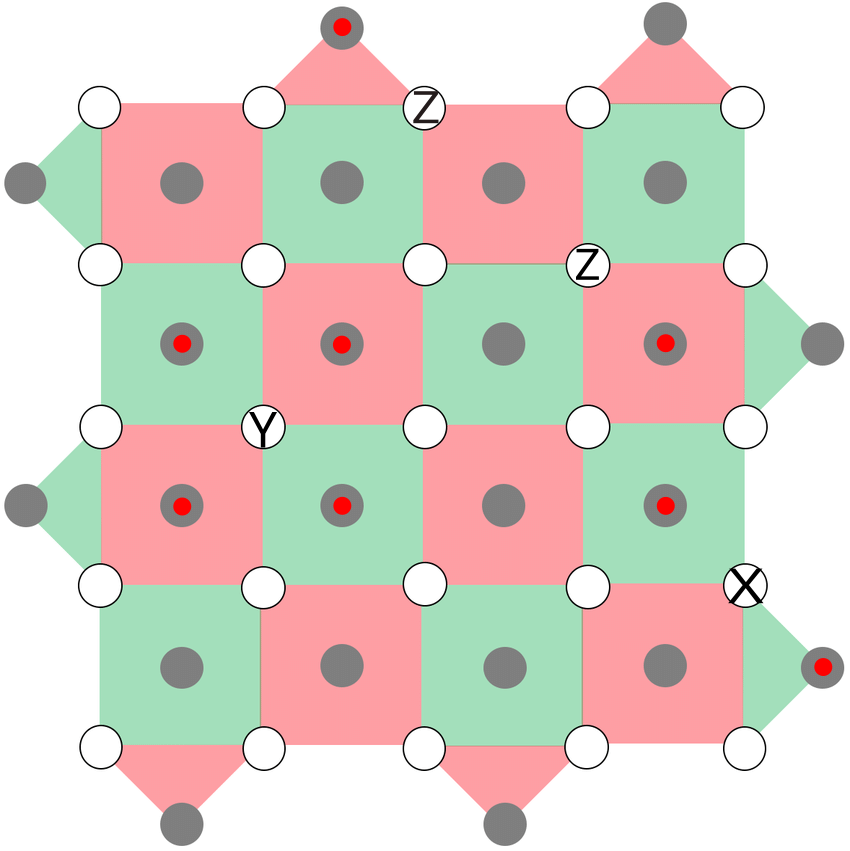
\includegraphics[scale=0.25]{./img/figures/d5surfaceCode.png}\\
	\caption{Distance 5 Surface code with data qubits in white and 
    ancilla qubits in grey. Green Faces represent Z stabilizers
    and Red faces represent X stabilizers.
    Errors on data qubits are marked
    by respective Pauli names and violated stabilizers are marked in red.}
	\label{fig: surface_code}
	\end{center}
\end{figure}
